\section{BC06 - Direction de projets de gestion de données}

\begin{frame}
    \centering
    \huge
    BC06 - Direction de projets de gestion de données
\end{frame}

\begin{frame}{Contexte et besoin métier}
	\textbf{Présentation du projet}\\
	\textit{GuitarFlow} est une entreprise développant un prototype de service d’intelligence artificielle destiné à la transcription automatique d’enregistrements audio de guitare en fichiers MIDI exploitables en MAO (Musique Assistée par Ordinateur).
	
	\vspace{0.3cm}
	
	\textbf{Constat métier}\\
	La retranscription manuelle d’une performance de guitare vers un format éditable constitue une tâche \textbf{chronophage}, nécessitant une \textbf{expertise musicale avancée} et difficilement \textbf{industrialisation-compatible} pour des usages pédagogiques ou créatifs.
	
	\vspace{0.3cm}
	
	\textbf{Opportunité}\\
	Le projet vise à :
	\begin{itemize}
		\item réduire le temps de transcription audio $\rightarrow$ MIDI,
		\item faciliter la production de contenus pédagogiques,
		\item accélérer les workflows de composition musicale,
		\item proposer un démonstrateur d’IA appliquée au signal audio.
	\end{itemize}
\end{frame}

\begin{frame}{Cadrage du projet}
    \textbf{Objectif principal}\\
    Développer un prototype de service capable de :
    \begin{itemize}
    	\item recevoir un fichier audio guitare,
    	\item générer automatiquement un fichier MIDI exploitable,
    	\item produire une visualisation de type piano-roll,
    	\item exposer le modèle via une API web déployée sur Hugging Face.
    \end{itemize}
    
    \vspace{0.3cm}
    
    \begin{minipage}[t]{0.48\textwidth}
    	\textbf{Fonctionnalités incluses}
    	\begin{itemize}
    		\item Audio guitare mono instrument
    		\item Guitare acoustique et électrique
    		\item Accordage standard (EADGBE)
    		\item Génération MIDI
    		\item Visualisation piano-roll
    		\item API REST d’inférence
    		\item Conteneurisation Docker
    	\end{itemize}
    \end{minipage}
    \hfill
    \begin{minipage}[t]{0.48\textwidth}
    	\textbf{Fonctionnalités hors périmètre}
    	\begin{itemize}
    		\item Multi-instruments
    		\item Accordages alternatifs
    		\item Temps réel
    		\item Techniques de jeu avancées
    		\item Application mobile native
    		\item Architecture cloud managée
    	\end{itemize}
    \end{minipage}
\end{frame}

\begin{frame}{Analyse des besoins et exigences}
    \textbf{Exigences fonctionnelles}\\
    \begin{itemize}
    	\item Accepter un enregistrement audio de guitare au format WAV.
    	\item Produire automatiquement une transcription au format MIDI exploitable dans un logiciel de MAO.
    	\item Permettre la visualisation des notes détectées sous forme de piano-roll.
    	\item Exposer le service via une API REST et une interface web.
    	\item Garantir la prise en charge d'enregistrements de guitare acoustique et électrique.
    	\item Permettre l'évaluation et la comparaison de plusieurs approches de transcription.
    \end{itemize}
    
    \vspace{0.3cm}
    
    \textbf{Exigences non fonctionnelles}\\
    \begin{itemize}
    	\item Temps d'inférence inférieur à 10 secondes pour 1 minute d'audio.
    	\item Reproductibilité complète des expérimentations et des résultats.
    	\item Traçabilité des jeux de données, modèles et métriques.
    	\item Déploiement reproductible par conteneurisation Docker.
    	\item Maintenabilité assurée par une architecture modulaire, des tests automatisés et une documentation technique.
    \end{itemize}
\end{frame}

\begin{frame}{Critères de succès}
	\centering
	\begin{tabular}{ll}
		\toprule
		\textbf{Indicateur} & \textbf{Objectif cible} \\
		\midrule
		F1-score de transcription polyphonique & $\geq 90\,\%$ \\
		Temps moyen d'inférence & $< 10$ s pour 1 min d'audio \\
		Disponibilité du prototype & Démonstration fonctionnelle avant le 31/07/2026 \\
		Déploiement & API accessible via une interface web \\
		Taux de correction manuelle & $< 10\,\%$ \\
		\bottomrule
	\end{tabular}
\end{frame}

\begin{frame}{Organisation et planification}
    \textbf{Approche de pilotage}\\
    Le projet a été conduit selon une démarche incrémentale articulée autour de quatre jalons de validation permettant de sécuriser progressivement les différentes phases du POC.
    
    \vspace{0.3cm}
    \centering
    
    \begin{tabular}{lll}
    	\toprule
    	\textbf{Jalon} & \textbf{Semaine} & \textbf{Critère de validation} \\
    	\midrule
    	J1 -- Go Datasets      & S4  & Données validées et exploitables \\
    	J2 -- Go Modèle        & S6  & Baseline opérationnelle \\
    	J3 -- Go Prototype     & S8  & Pipeline complet exécutable \\
    	J4 -- Go Démonstration & S10 & API et interface accessibles \\
    	\bottomrule
    \end{tabular}
    
    \vspace{0.3cm}
    
    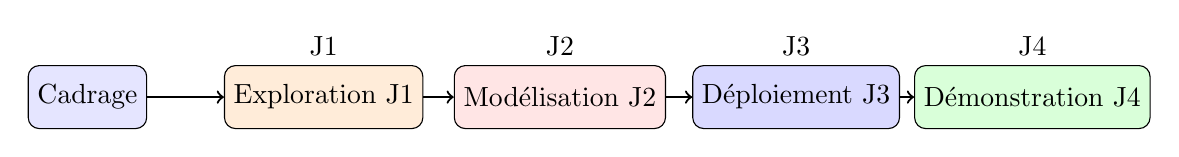
\begin{tikzpicture}
    	[phase/.style={rectangle, draw, rounded corners, minimum height=0.8cm, align=center}]
    	
    	\node[phase, fill=blue!10] (c) at (0,0) {Cadrage};
    	\node[phase, fill=orange!15] (e) at (3,0) {Exploration J1};
    	\node[phase, fill=red!10] (m) at (6,0) {Modélisation J2};
    	\node[phase, fill=blue!15] (d) at (9,0) {Déploiement J3};
    	\node[phase, fill=green!15] (f) at (12,0) {Démonstration J4};
    	
    	\draw[->, thick] (c) -- (e);
    	\draw[->, thick] (e) -- (m);
    	\draw[->, thick] (m) -- (d);
    	\draw[->, thick] (d) -- (f);
    	
    	\node[above] at (3,0.4) {J1};
    	\node[above] at (6,0.4) {J2};
    	\node[above] at (9,0.4) {J3};
    	\node[above] at (12,0.4) {J4};
    \end{tikzpicture}
    
    \vspace{0.3cm}
    
    \hyperlink{gantt}{\beamergotobutton{Voir le Gantt détaillé}}
\end{frame}

\begin{frame}{Analyse des risques}
	\centering
	\begin{tabular}{p{5.4cm} l l p{5.4cm}}
		\toprule
		\textbf{Risque} & \textbf{Impact} & \textbf{Prob.} & \textbf{Mitigation} \\
		\midrule
		Restrictions de licence sur les datasets & Élevé & Moyen & Validation juridique des sources avant intégration \\
		Volume de données insuffisant & Élevé & Élevé & Data augmentation + transfer learning \\
		Performances insuffisantes en polyphonie & Élevé & Moyen & Benchmark de plusieurs architectures (baseline / CNN / CRNN) \\
		Temps d’inférence trop élevé & Moyen & Moyen & Optimisation du modèle + quantization \\
		Variabilité de qualité audio & Moyen & Élevé & Normalisation et standardisation du signal audio \\
		\bottomrule
	\end{tabular}
\end{frame}

\begin{frame}{Architecture cible}
	\begin{figure}[h]
		\centering
		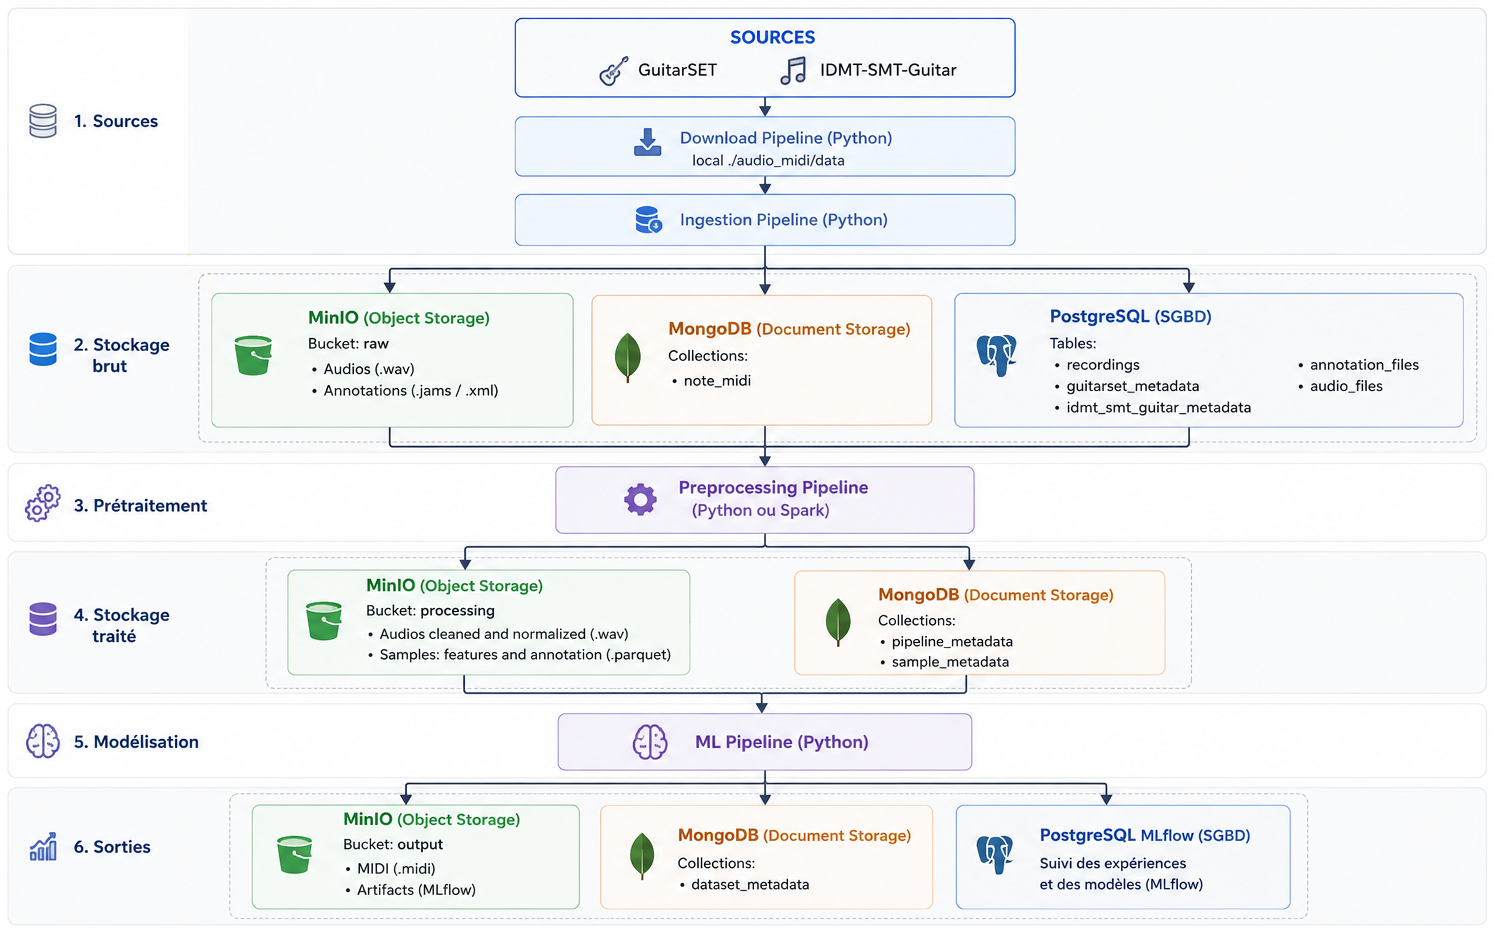
\includegraphics[width=0.7\textwidth]{figures/BC01/architecture_globale.png}
		% \caption{Architecture cible}
		\label{fig:architecture_cible}
	\end{figure}
\end{frame}

\begin{frame}{Réalisation du POC}
	\textbf{Approche de réalisation}\\
	Le POC a été construit selon une logique de pipeline end-to-end couvrant l’ensemble du cycle de vie de la donnée : ingestion, traitement, entraînement et mise à disposition du modèle.
	
	\vspace{0.3cm}
	
	\textbf{Livrables techniques}\\
	\begin{itemize}
		\item Pipeline d’ingestion des données (GuitarSet, IDMT-SMT-Guitar)
		\item Pipeline de prétraitement audio et extraction de caractéristiques
		\item Pipeline d’entraînement et d’évaluation des modèles
		\item Modèle entraîné et évalué pour la transcription audio $\rightarrow$ MIDI
		\item API REST d’inférence (FastAPI)
		\item Conteneurisation du système via Docker / Docker Compose
		\item Interface de démonstration déployée sur Hugging Face Spaces
	\end{itemize}
	
	\vspace{0.3cm}
	
	\textbf{Livrables documentaires}\\
	\begin{itemize}
		\item Note de cadrage et cahier des charges
		\item Documentation technique des pipelines et de l’architecture
		\item Guide d’installation et de déploiement
		\item Support de présentation pour la soutenance
	\end{itemize}
\end{frame}

\begin{frame}{Résultats obtenus}
	\textbf{Performance du système}\\
	\centering	
	\begin{tabular}{l c}
		\toprule
		\textbf{Indicateur} & \textbf{Résultat} \\
		\midrule
		F1-score transcription polyphonique & xx \% \\
		Temps d’inférence moyen & xx s pour 1 min d’audio \\
		Génération de fichier MIDI & Oui \\
		Visualisation piano-roll & Oui \\
		API d’inférence fonctionnelle & Oui \\
		\bottomrule
	\end{tabular}
	
	\vspace{0.3cm}
	
	\textbf{Exemple de sortie du modèle}\\
	\begin{itemize}
		\item Conversion automatique d’un extrait audio en fichier MIDI exploitable
		\item Reconstruction des notes jouées sur guitare (mono et polyphonique)
		\item Visualisation synchronisée type piano-roll
	\end{itemize}
	
	\vspace{0.3cm}
	
	\begin{bloc}
		Le POC démontre la faisabilité technique et la valeur métier de la transcription audio $\rightarrow$ MIDI.
	\end{bloc}
\end{frame}

\begin{frame}{Gouvernance et qualité}
    Cette slide fait souvent la différence.

    Contenu :
    - Git
    - Docker
    - MLflow
    - Versionning datasets
    - Reproductibilité

    Message clé :
    Maîtrise du cycle de vie du projet.
\end{frame}

\begin{frame}{Bilan et perspectives}
    Bilan :
    - Faisabilité validée
    - Prototype opérationnel
    
    Perspectives :
    - Industrialisation
    - API dédiée
    - Temps réel
    - Généralisation multi-instruments

    Message clé :
    Projection vers une phase produit.
\end{frame}